% !TEX program = lualatex

\documentclass[final]{beamer}

% ====================
% Packages
% ====================
% \usepackage[T1]{fontenc}
% \usepackage{lmodern}
\usepackage{fontspec}
\setsansfont{Roboto}
\setmainfont{Roboto}
\newfontfamily\bookerlyfont{bookerly}
\usepackage[orientation=portrait,size=a0,scale=1.1]{beamerposter}
\usetheme{gemini}
\usecolortheme{rose}  % options: mit, kyb
\usepackage{amsmath}
\usepackage{amssymb}
\usepackage{amsfonts}
\usepackage{dsfont}
\usepackage{xcolor}
\usepackage{pgfplots}
\pgfplotsset{compat=1.14}
\usepackage{graphicx}
\usepackage{array}
\usepackage{booktabs}
\usepackage{qrcode}
\usepackage{anyfontsize}
\usepackage{svg}
\usepackage{subcaption}
\usepackage[italicdiff]{physics}
\usepackage[absolute,overlay]{textpos}
\usepackage[backend=biber, style=numeric, sorting=none, natbib=true]{biblatex}
\addbibresource{poster.bib} % This loads your new poster.bib file
% ====================
% custom commands
% ====================
\newcommand{\mpl}{M_{\text{Pl}}^2}
\newcommand{\lcdm}{$\Lambda$CDM }

% ====================
% Lengths
% ====================
\usebackgroundtemplate{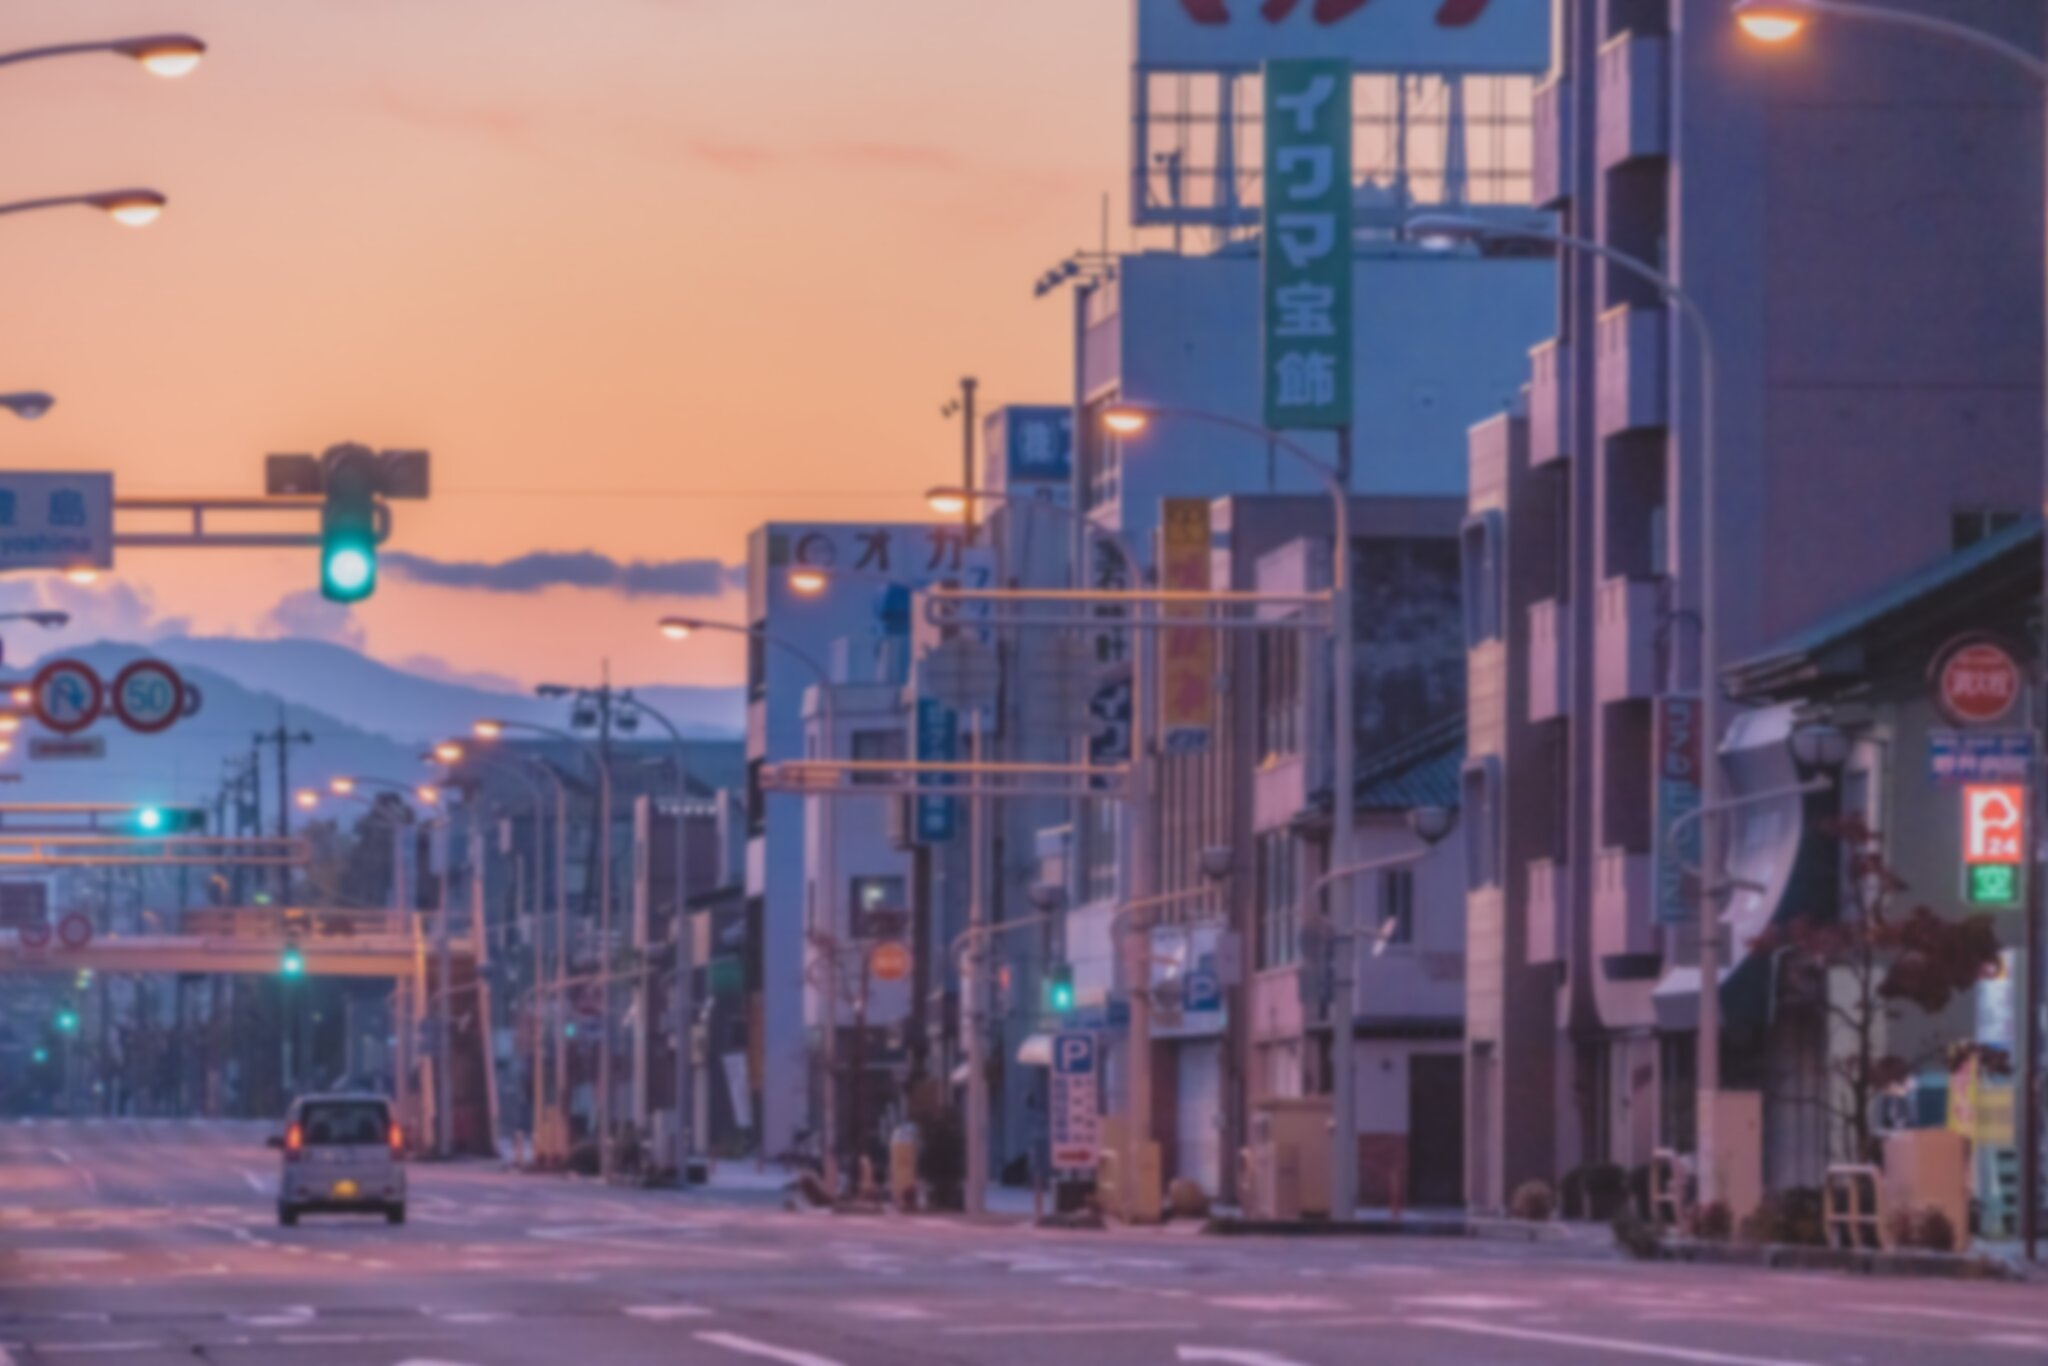
\includegraphics[height=\paperheight]{Backgrounds/active_background}}

\newlength{\sepwidth}
\newlength{\colwidth}
\setlength{\sepwidth}{0.05\paperwidth}
\setlength{\colwidth}{0.425\paperwidth}
\setlength{\maxlogowidth}{0.2\paperwidth}

\newcommand{\separatorcolumn}{\begin{column}{\sepwidth}\end{column}}
\newcommand{\apjs}{Astrophys. J. Suppl. Ser.}

\usepackage[most]{tcolorbox}

% ====================
% Title
% ====================

\title{Model selection with neural networks \\ and clustering data from simulations}

\author{\textbf{Charlotte Guajardo-Martínez}\inst{1} \and Indira Ocampo\inst{2} \and Domenico Sapone\inst{1}}

\institute[shortinst]{
 \inst{1} Departamento de Física, FCFM, Universidad de Chile, Santiago, Chile.\\
 \vspace{2pt}
 \inst{2} Instituto de Física Teórica UAM/CSIC, Madrid, Spain.
}
% ====================
% Footer
% ====================

\footercontent{ 
  \bookerlyfont \textbf{Cosmosur VIII} \hfill \href{mailto:charlotte.guajardo@ug.uchile.cl}{$^1$ \textbf{charlotte.guajardo@ug.uchile.cl} \quad
\qrcode[height=1in]{https://charlotteguajardo.github.io/}} 
}

\begin{document}

% ====================
% Logos
% ====================

\begin{textblock*}{0.85\paperwidth}(0.07\paperwidth,0.04\paperheight)
  \centering
  \raisebox{1cm}{
\includegraphics[height=5cm]{logos/dfi_white.pdf}}\hfill
  
\includegraphics[height=7cm]{logos/cosmouchile_white_v2.pdf}
\end{textblock*}

% ====================
% Body
% ====================

\begin{frame}[t]

%========================================

\begin{columns}[t]
\separatorcolumn
  \begin{column}{\dimexpr2\colwidth+\sepwidth\relax}
  \begin{block}{Motivation}
    In 2024, the DESI survey observations indicated a preference for dynamical dark energy models over standard \lcdm \cite{adame2025desi}. In the search for additional ways to validate or discard cosmological models using observational data, \cite{ocampo2025enhancing} uses neural networks trained with mock growth rate data as likelihood-free model selection tool. We aim to expand on this analysis by including simulation measurements and a full-shape analysis of $P_m(k)$.
\end{block}
  \end{column}
\separatorcolumn
\end{columns}

%========================================

\begin{columns}[t]
\separatorcolumn

\begin{column}{0.75\colwidth}
\begin{block}{Full shape and growth rate}
Changes in cosmology can noticeably affect the matter power spectrum. It can change the peak position, slope, or growth history. For that reason, we can approach the task of model selection using the full-shape at redshift $z=0$ or the growth of structure.\\

For the growth history analysis, we can use the growth rate $f\sigma_{8}(z)$, where $f(z) \equiv \dd{\ln\delta_+}/\dd{\ln{a}}$. It is common to fit this parameter as

\begin{equation}
  f(z) = \Omega_m^\gamma(z)\text{,}
\end{equation}

where $\gamma$ is sensitive to changes in the cosmological model and is $\approx 0.55$ for $\Lambda$CDM\\


\end{block}
\end{column}

% \separatorcolumn
\begin{column}{0.5\sepwidth}\end{column}

\begin{column}{1.3\colwidth}
  \begin{block}{Modified Gravity and Simulations}
\vspace{-3ex}
  \begin{columns}[t]
    \begin{column}{0.47\linewidth}
      \justify
      The $f(R)$ self-accelerated gravity models replace the cosmological constant in Hilbert-Einstein action in the following way:\\
      \begin{equation}
  S = \int d^4x\sqrt{-g}\Big( \frac{R+f(R)}{2\kappa^2} + \mathcal{L}_m \Big)\text{.}
\end{equation}
      The Hu-Sawicki gravity (HS) is particularly useful for clustering comparisons, since \textbf{it shares the same background history} as $\Lambda$CDM, and its deviation from it can be parameterized with a single constrainable value: $f_{R0}$
      
      \begin{equation}
        f(R)=-6 \Omega_{\mathrm{DE}, 0} \frac{H_0^2}{c^2}+\left|\boldsymbol{f_{R 0}}\right| \frac{\bar{R}_0^2}{R}+\ldots
      \end{equation}
    \end{column}
    
    
    \hfill % Automatically creates an even gap between the two columns
    
    \begin{column}{0.47\linewidth}
      \justify
      We use the \textbf{Quijote Simulations} \cite{Quijote_sims} suite of N-body simulations for machine learning to obtain $P(k)$ measurements and their covariances for 2048 combinations of these parameters.

      
      \begin{columns}[T]
        \begin{column}{0.48\linewidth}
          \vspace{0pt}
          \begin{table}
            \centering
            \renewcommand{\arraystretch}{1.2}
            $\begin{array}[t]{r c l}
              \Omega_{\mathrm{m}} & \in & [0.10; 0.50] \\
              \Omega_{\mathrm{b}} & \in & [0.03; 0.07] \\
              h & \in & [0.50; 0.90] \\
              n_s & \in & [0.80; 1.20] \\
              \sigma_8(GR) & \in & [0.60; 1.00] \\
              f_{R0} & \in & [-3 \times 10^{-4}; 0]
            \end{array}$
            \caption{Parameters for the HS simulations.}
          \end{table}
        \end{column}
        
        \begin{column}{0.48\linewidth}
          \vspace{0pt}
          \begin{table}
            \centering
            \renewcommand{\arraystretch}{1.2}
            $\begin{array}[t]{r c l}
              \Omega_{\mathrm{m}} & \in & [0.10; 0.50] \\
              \Omega_{\mathrm{b}} & \in & [0.02; 0.08] \\
              h & \in & [0.50; 0.90] \\
              n_s & \in & [0.80; 1.20] \\
              \sigma_8 & \in & [0.60; 1.00]\\
              &&
            \end{array}$
            \caption{Parameters for the \lcdm simulations.}
          \end{table}
        \end{column}
      \end{columns}
      
      
    \end{column}
  \end{columns}
\vspace{-1.2ex}
\end{block}
    
\end{column}
\separatorcolumn
\end{columns}

%================================================

\begin{columns}[t]
\separatorcolumn
\begin{column}{0.66\colwidth}
\begin{block}{Building the growth rate}
The growth factor $\delta_+$ of perturbations is scale dependent in HS, so we take its value at $k_t = 0.1$ h/Mpc.
\vspace{0ex}
\begin{equation}
    \delta_+(a) = \sqrt{P(k_t,a)/P(k_t,a=1)}\text{.}
\end{equation}

Then, to perform the logarithmic derivative, we fit it to 2nd degree polynomial, obtaining:

\begin{equation}
    a\delta_+'(a) = \delta_+(a)\dv{\ln\delta_+(a)}{\ln{a}} = f\sigma_8(a)/\sigma_{8,0}\text{.}
\end{equation}


\end{block}
\end{column}

\begin{column}{0.5\sepwidth}\end{column}

\begin{column}{0.66\colwidth}
\begin{block}{Building The Neural Network}
  We use our growth rate and power spectra measurements to train a neural network for binary classification. The architecture of the model is a standard multi-layer perceptron, with three hidden layers and a $50\%$ Dropout. We also included:

  \begin{itemize}
    \item \textbf{Optuna}: For hyperparameter tuning.
    \item \textbf{L1 regularization}: For generalization and contrast increase on the feature importance analysis.
  \end{itemize}
\end{block}
\end{column}

\begin{column}{0.5\sepwidth}\end{column}


\begin{column}{0.66\colwidth} 
  \begin{block}{}
  \begin{figure}[h]
      \centering
      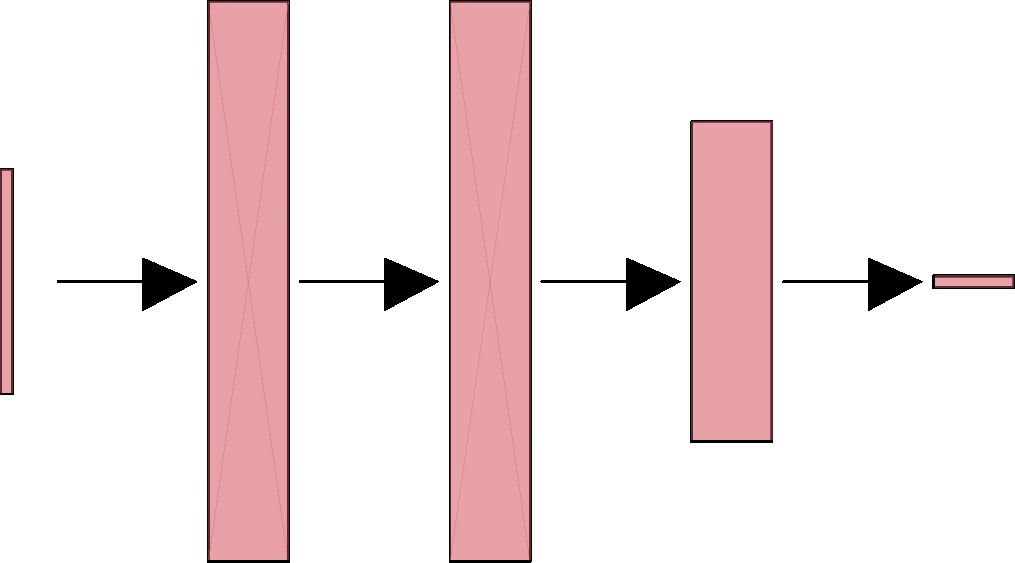
\includegraphics[width=0.83\textwidth]{figures/nn.pdf}
      \caption{General architecture of the NN models used.}
  \end{figure}
\end{block}
\end{column}
\separatorcolumn
\end{columns}

%========================================

\begin{columns}[t]
\separatorcolumn

  \begin{column}{1.025\colwidth}
  \begin{block}{Neural Network Training and Performance}

To train the neural networks, we add noise to the data using their respective covariance matrices. We obtain very accurate results from both approaches, with the full-shape model performing considerably better.\\

    \begin{figure}[h]
        \centering
        \begin{subfigure}{0.42\textwidth}
            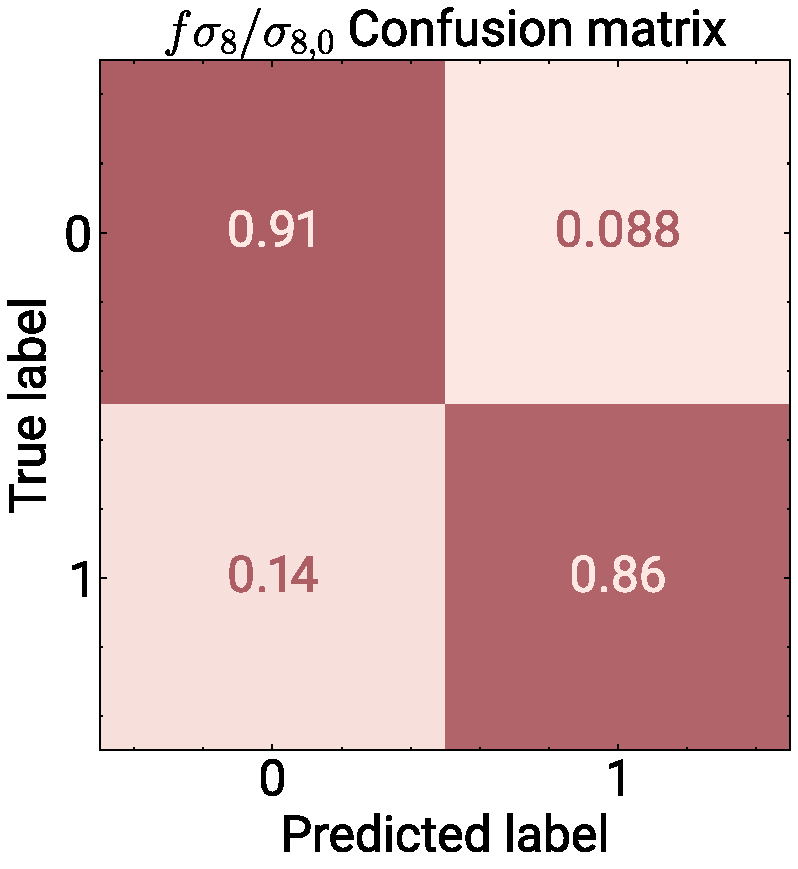
\includegraphics[width=\textwidth]{figures/fs8_cm.pdf}
        \end{subfigure}\hfill
        \begin{subfigure}{0.42\textwidth}
            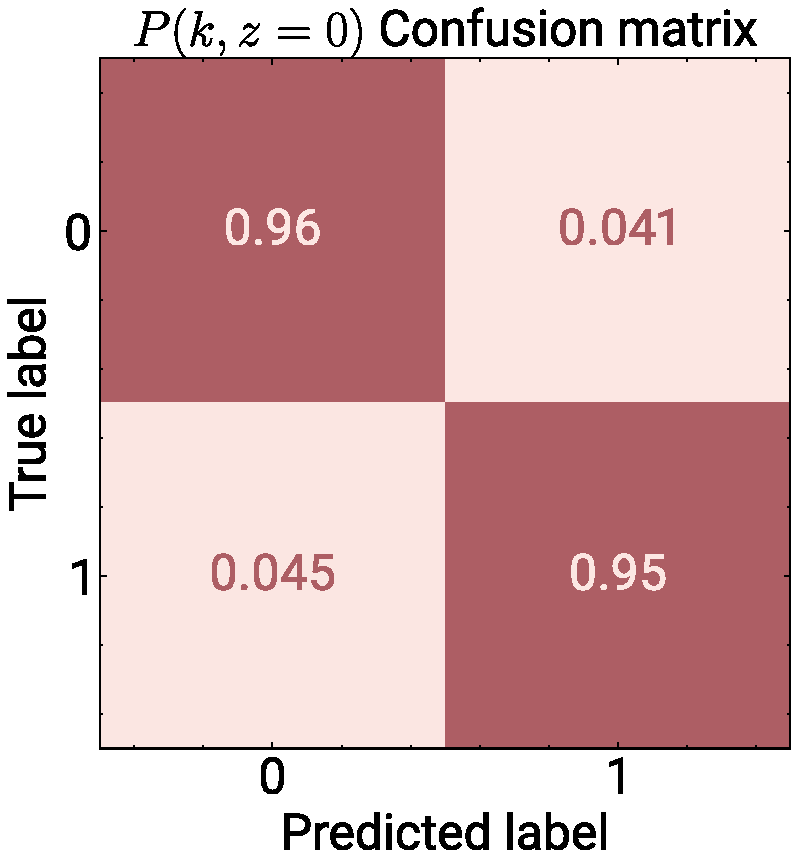
\includegraphics[width=\textwidth]{figures/Pk_cm.pdf}
        \end{subfigure}
        \caption{Confusion matrix for both models, where 0 is the label for \lcdm and 1 for HS.}
    \end{figure}
\vspace{3ex}
\end{block}
 

  \end{column}

  \begin{column}{0.5\sepwidth}\end{column}
  
  \begin{column}{1.025\colwidth}
  \begin{alertblock}{What is the model looking at?}
Using the feature analysis tool Shap \cite{lundberg2017unified}, we find that:
\begin{itemize}
  \item Not only low redshifts measurements are relevant for predictions based on growth rate.
  \item The models values the $P(k)$ derivatives at quasi non-linear and non-linear scales over the peak position
\end{itemize}.
\vspace{-2ex}
 \begin{figure}[h]
   \centering
   \begin{subfigure}{0.48\textwidth}
     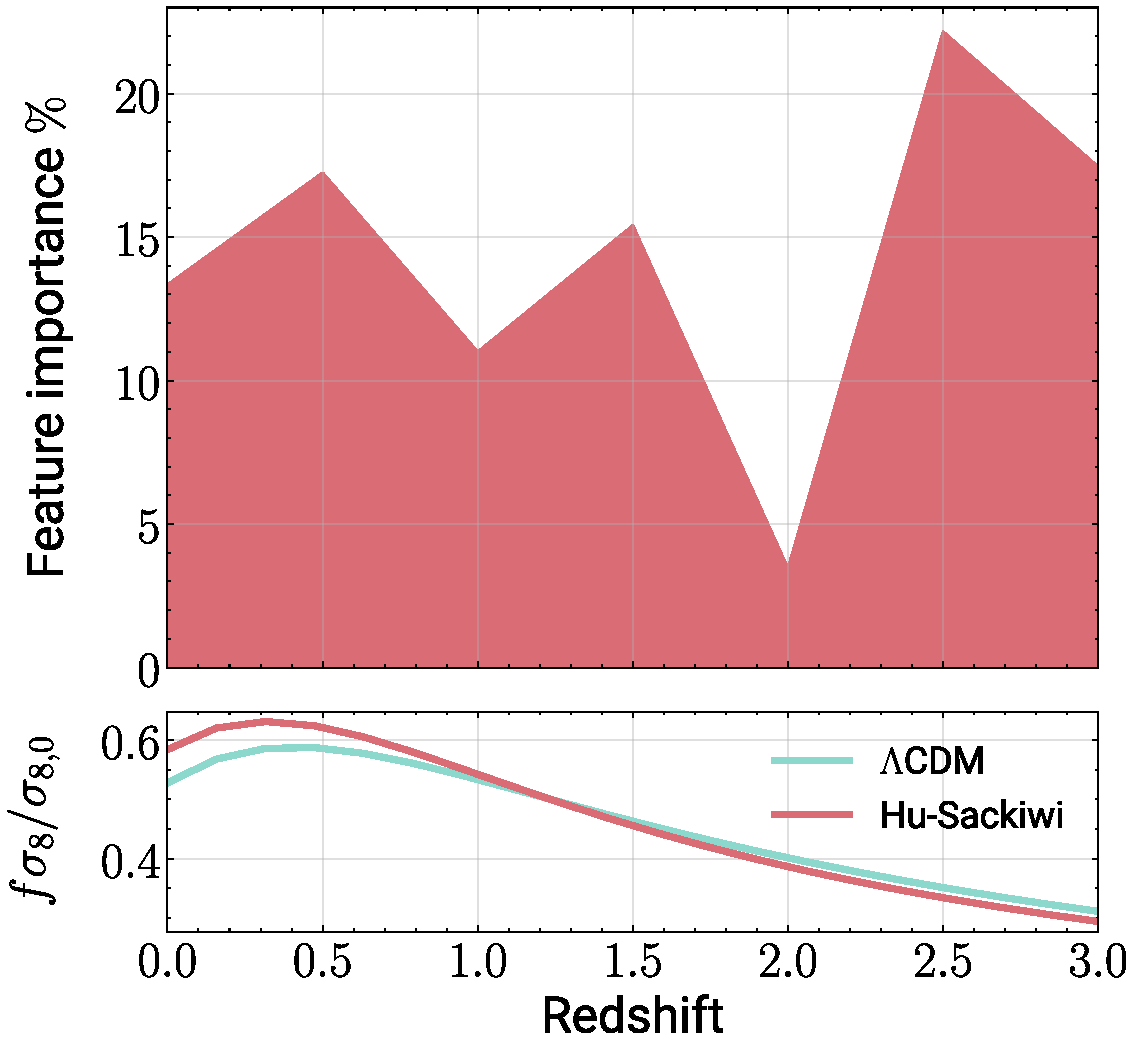
\includegraphics[width=\textwidth]{figures/fs8_features.pdf}
     
   \end{subfigure}\hfill
   \begin{subfigure}{0.477\textwidth}
     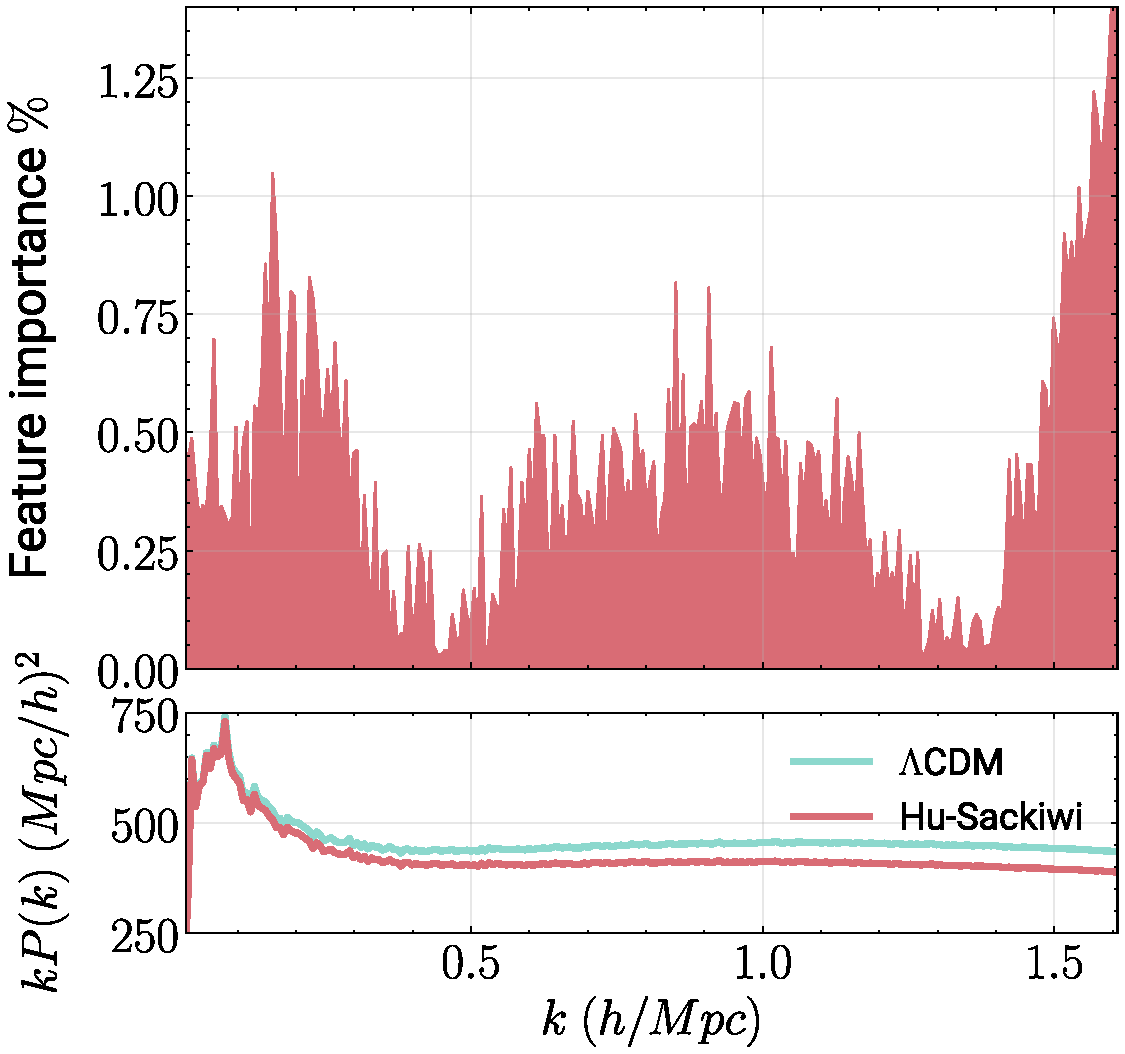
\includegraphics[width=\textwidth]{figures/pk_features.pdf}

   \end{subfigure}
   \caption{Feature analysis compared to MGCAMB results for reference.}
 \end{figure}

\end{alertblock}
  \end{column}

\separatorcolumn
\end{columns}

%========================================

\begin{columns}[t]
\separatorcolumn

  \begin{column}{0.8\colwidth}
  \begin{block}{Conclusions}
  \begin{itemize}
    \item Neural networks are capable of accurately discern between models using the full shape $P(k)$ and its growth history.
    \item Feature analysis reflects some of the expected physical mechanisms present in the clustering measurements.
  \end{itemize}

\end{block}
  \end{column}

  \begin{column}{0.5\sepwidth}\end{column}
  \begin{column}{0.4\colwidth}
  \begin{block}{Acknowledgments}
    This work wouldn't be possible without the financial support of the Fondecyt regular 1251339.
\vspace{3ex}
\end{block}
  \end{column}
  \begin{column}{0.5\sepwidth}\end{column}
  \begin{column}{0.8\colwidth}
\begin{block}{References}
  \renewcommand*{\bibfont}{\fontsize{18}{18}\selectfont}
  \printbibliography[heading=none]
\end{block}
  \end{column}
  
  
\separatorcolumn
\end{columns}



\end{frame}
\end{document}
